\documentclass[a4paper, 14pt,russian]{extarticle}

\usepackage[russian]{babel}
\usepackage[T2A]{fontenc}
\usepackage[utf8]{inputenc}
%Соответствующий математический шрифт для Times new roman
\usepackage{newtxmath}
\usepackage{fontspec} 
%Times new roman
\defaultfontfeatures{Ligatures={TeX},Renderer=Basic} 
\setmainfont[Ligatures={TeX,Historic}]{Times New Roman}

%Геометрия
\usepackage{geometry}
\geometry{top=20mm}
\geometry{bottom=15mm}
\geometry{left=20mm}
\geometry{right=15mm}
\usepackage{setspace}
%Нормальные дроби через запятую
\usepackage{ncccomma}

\newcommand{\changefont}{%
	\fontsize{12}{11}\selectfont
}
\newcommand{\normE}[1]{
	\lvert\lvert {#1} \rvert\rvert_2
}

%Заголовки
\usepackage{fancyhdr}
%\pagestyle{fancy}
%\fancyhf{}
%\renewcommand{\sectionmark}[1]{\markright{#1}}
%\fancyhead[R]{\changefont \slshape \leftmark}
%\fancyhead[L]{\changefont \slshape \rightmark}
%\newcommand{\ssubsection}[1]{\subsection*{#1}
%	\addcontentsline{toc}{subsection}{#1}
%	\markright{#1}{}}
\cfoot{\thepage}

%\полуторный интервал
\setstretch{1.15}
\setlength{\parindent}{1.25cm}

\usepackage{amsmath, amsfonts, mathtools}
\usepackage{physics}
\usepackage{indentfirst}
\usepackage{xcolor}
\usepackage{alltt}
\usepackage{graphicx}
\usepackage{wrapfig}
%Настройка ссылок
\usepackage{hyperref}
%\usepackage{upgreek}
%\renewcommand{\beta}{\upbeta}
\hypersetup{
	colorlinks,
	citecolor=black,
	filecolor=black,
	linkcolor=black,
	urlcolor=black
}
\usepackage{caption}
\DeclareCaptionLabelSeparator{dot}{. }
\captionsetup{justification=centering,labelsep=dot}
\usepackage{titlesec}

%Формат заголовков
\titleformat{\section}{\bfseries\filcenter\Large}{\thesection}{1em}{}
\titleformat{\subsection}{\bfseries\filcenter\large}{\thesubsection}{1em}{}
\titleformat{\subsubsection}{\bfseries\filcenter\normalsize}{\thesubsubsection}{1em}{}

\usepackage{chngcntr}

%Включить в нумерацию картинок раздел
\counterwithin{figure}{section}

%Листинги кода и их стили
\usepackage{listings}
\lstdefinestyle{c++} {
	language=C++,
	breaklines=true,
	frame=single,
	numbers=left,
	basicstyle=\footnotesize\ttfamily,
	keywordstyle=\bfseries\color{green!40!black},
	commentstyle=\itshape\color{purple!40!black},
	identifierstyle=\color{blue},
	backgroundcolor=\color{gray!10!white},
}

\lstdefinestyle{python}{
	language=Python,
	breaklines=true,
	frame=single,
	numbers=left,
	basicstyle=\footnotesize\ttfamily,
	keywordstyle=\bfseries\color{green!40!black},
	frame=lines
	basicstyle=\footnotesize
}

\lstdefinestyle{cmd}{
	breaklines=true,
	frame=single,
	basicstyle=\footnotesize\ttfamily,
	frame=lines
	basicstyle=\footnotesize
}

\begin{document}
	
	\begin{titlepage}
	\newpage
	\begin{center}
		
\includegraphics[width=\textwidth]{tit.png}
		Институт информационных и вычислительных технологий \\
			Кафедра управления и интеллектуальных технологий
		\vspace{1.25cm}
	\end{center}
	
	\vspace{1.2em}
	
	\begin{center}
		%\textsc{\textbf{}}
		\begin{spacing}{1}
			{\Large \textbf{ Прогноз энергетики: теоретическая справка по статистическим методам прогноза} \\}
			\vspace{1em}
			{ \large \textbf{Михайловский Михаил, А-03-21}\\}
			\vspace{0.3em}
			{Промежуточная версия от 21.04.24}
			
		\end{spacing}
	\end{center}
	
	\vspace{6em}
	

	\vspace{6em}
	
	
	\vspace{\fill}
	
	\begin{center}
		Москва 2024
	\end{center}
	
\end{titlepage}
	
	\pagenumbering{arabic}
	\setcounter{page}{2}
	
	\tableofcontents
	\newpage
	
	\section{Линейная регрессия}
	\subsection{Постановка задачи}
	
	Имеется некоторая выборка входных параметров и предсказываемого значения: $\{\vec{x}_j, y_j\}_{j=1}^N$. Здесь $\vec{x}_j^\intercal = [x_j^{(1)}\,\dots\,x_j^{(M)}]$ -- некоторый набор параметров, по которому требуется характеризовать предсказываемый параметр $y_j$.
	
	Нужно найти линейную зависимость $\hat{f}(\vec{x})$, которая по входным параметрам $\vec{x}_j^\intercal$ даст оценку $\hat{y}_j$ предсказываемого параметра $y_j$, следующего вида:
	\begin{equation*}
		\hat{y}_j = \hat{f}(\vec{x}_j) = \hat{b}_0 + \hat{b}_1x_j^{(1)}+ \dots + \hat{b}_M x_j^{(M)} = \vec{\hat{b}}^\intercal \vec{x}_j,\;\text{где }\vec{\hat{b}}^\intercal = [\hat{b}_0\;\hat{b}_1\;\dots\; \hat{b}_m]
	\end{equation*}
	При этом, $\hat{f}(\vec{x})$ является оценкой реальной зависимости $y_j = f(\vec{x}_j)\approx \hat{f}(\vec{x}_j)$.

	\subsection{Предположения метода}
	
	Следующие предположения в реальных условиях часто не выполняются. Поэтому их влияние стоит учитывать при анализе результатов. Есть метода для анализа выполнения этих предположений.
	\begin{enumerate}
		\item Истинное значение $y_j = f(\vec{x}_j) + e_j$, где $e_j$ -- аддитивная нормальная выходная помеха со следующими статистическими параметрами:
		\begin{equation*}
			e_j\sim N(0, \sigma_e),\;\sigma_e = \mathrm{const},\;\mathrm{cov}(e_j, e_k)=0
		\end{equation*} 
		\item Входные величины $x_j$ являются детерминированными и линейно независимыми.
	\end{enumerate}
	
	\subsection{Метод множественной линейной регрессии и его интерпретация}
	
	Для нахождения $\hat{f}(\vec{x}) = \vec{\hat{b}}^\intercal\vec{x}$ нужно найти $\vec{\hat{b}}$.
	
	\begin{equation*}
		\vec{\hat{b}} = \left(X^\intercal X\right)^{-1}X^\intercal \vec{y},\;\text{где }X = \begin{bmatrix*}
			1 & x_1^{(1)} & x_1^{(2)} & \dots & x_1^{(M)} \\
			1 & x_2^{(1)} & x_2^{(2)} & \dots & x_2^{(M)} \\
			\dots & \dots & \dots & \dots & \dots \\
			1 & x_N^{(1)} & x_N^{(2)} & \dots & x_N^{(M)}
		\end{bmatrix*}
	\end{equation*}
	
	Математически такая оценка вектора $\vec{b}$ является решением следующей оптимизационной задачи:
	
	\begin{equation*}
		MSE = \normE{\vec{y} - X\vec{b}}^2 = \sum_{j=1}^N\left(y_j - \vec{b}^\intercal\vec{x}_j\right)^2 \to \min_{\vec{b}\in\mathbb{R}^M}
	\end{equation*}

	Графически через набор наблюдений проводится прямая, имеющая в среднем минимальное отклонение от набора наблюдений (рис. \ref{graph}).
	
	\begin{figure}[h]
		\centering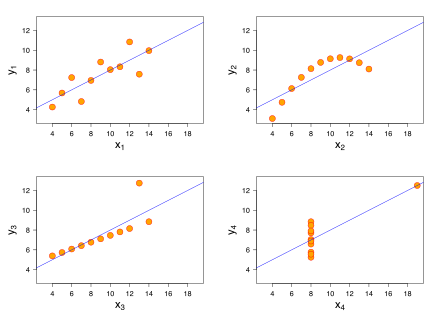
\includegraphics[width=.8\textwidth]{png/interpret.png}
		\caption{Графическая интерпретация для $M=1$}
		\label{graph}
	\end{figure}

	\textbf{Важные моменты.} Такой метод структурно не может работать точно, если зависимость $y(\vec{x})$ нелинейная (пример 2 на рисунке). Также, из-за вида критерия оптимизации метод ярко реагирует на выбросы. То есть даже небольшое количество значений, сильно отличающихся от основной массы, могут значительно изменить результат регрессии (пример 3 на рисунке).
	
	\subsection{Оценка адекватности модели}
	
	Для оценки адекватности можно использовать скорректированный коэффициент детерминации $R^2_{\text{корр}}$. Он рассчитывается с помощью:
	\begin{equation*}
		S_\text{ост}^2 = \frac{1}{N-(M-1)}\normE{\vec{\hat{y}} - \vec{y}}^2,\;\; S_\text{общ}^2 = \frac{1}{N-1}\normE{\vec{y} - X\vec{b}}^2,
	\end{equation*}
	\begin{equation*}
		R^2_\text{корр} = 1- \frac{S_\text{ост}^2}{S_\text{общ}^2}
	\end{equation*}
	
	При $R^2_\text{корр} \geq 0,75$ модель можно считать адекватной. Чем значение скорректированного коэффициента детерминации ближе к 1, тем лучше. С помощью этого коэффициента можно сравнивать модели с разным значением $M$.
	
	\section{Метод наименьших квадратов для прогноза временных рядов}
	\subsection{Задача прогноза временных рядов}
	
	Для прогноза значений временных рядов может быть использован метод наименьших квадратов (МНК). Обычный вид временных рядов представлен на рис. \ref{vr}. Это зависимость некоторого показателя $y(t)$. В отличие от рассмотренной постановки задачи для линейной регрессии здесь наблюдения упорядочены по времени отсчёта.
	
	\begin{figure}[h]
		\centering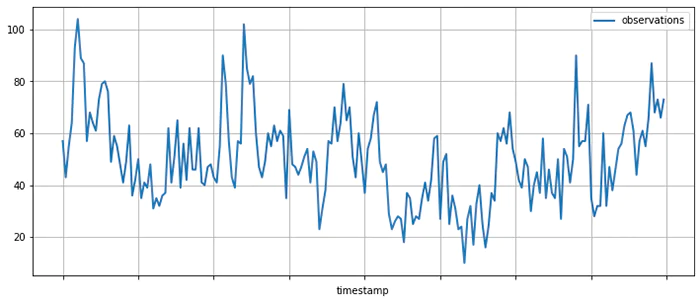
\includegraphics[width=.7\textwidth]{png/временной_ряд.png}
		\caption{Пример временного ряда}
		\label{vr}
	\end{figure}
	
	Такой ряд можно разбить на низкочастотную составляющую -- тренд и высокочастотную составляющую -- шум. Для получения тренда можно использовать метод скользящего среднего. При некоторых параметрах скользящее среднее даёт результат, как на рис. \ref{moveing_average}. Красная кривая является приближением к общему тренду временного ряда.
	
	\begin{figure}[h]
		\centering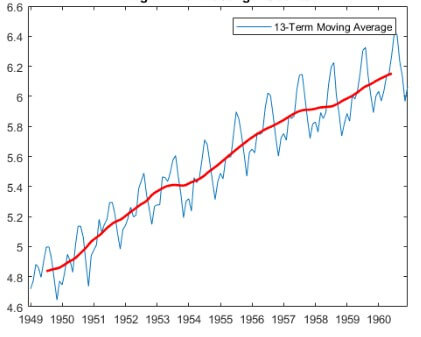
\includegraphics[width=.5\textwidth]{png/moving_average.jpg}
		\caption{Пример выделения тренда методом скользящего среднего}
		\label{moveing_average}
	\end{figure}

	Если шум является пренебрежимо малым относительно составляющей тренда, то в качестве предсказания можно ограничиваться лишь трендом. Для этого и используется метод МНК. Если шумом нельзя пренебречь, то можно отдельно изучать его статистические характеристики, проверить предположение на нормальность, и для нормального шума можно строить доверительные интервалы его значений. То есть можно указать интервал, в котором находится это значение с заданной исследователем вероятностью (обычно 95\%).
	
	\subsection{Постановка задачи метода наименьших квадратов}
	
	\textbf{Даны} узловые значения $\{x_i\}_{i=0}^N$ и значения функции в них $\{y_i\}_{i=0}^N$. 
	
	\textbf{Найти} функцию $\Phi_m(x):\;\Phi_m(x_i)\approx y_i \;\forall i$.
	
	При этом структура этой функции задаются следующим образом:
	\begin{equation*}
		\Phi_m(x) = a_0\varphi_0(x) + a_1\varphi_1(x) +\dots+a_m\varphi_m(x) = \sum_{j=0}^m a_j \varphi_j(x)
	\end{equation*}
	Набор функций $\{\varphi_i(x)\}_{i=0}^m$ задаётся исследователем.
	
	\subsection{Решение по методу МНК}
	
	Пусть набор функций $\{\varphi_i(x)\}_{i=0}^m$ уже задан. Тогда, для заданного набора узлов и значений в них неизвестные коэффициенты $a_j$ в функции $\Phi_m(x) = \sum_{j=0}^m a_j\varphi_j(x)$ можно найти из следующей системы алгебраических линейных уравнений:
	\begin{equation*}
		M\vec{a} = \vec{b},\; \vec{a} = \begin{bmatrix*}
			a_0 \\ a_1 \\ \dots \\ a_m
		\end{bmatrix*},\; \vec{b} = \begin{bmatrix*}
			\sum_{i=0}^N y_i\varphi_0(x_i) \\ \sum_{i=0}^N y_i\varphi_1(x_i) \\ \dots \\ \sum_{i=0}^N y_i\varphi_m(x_i)
	\end{bmatrix*}
	\end{equation*}
	\begin{equation*}
		M = \begin{bmatrix*}
			\sum_{i=0}^N \varphi_0(x_i)\varphi_0(x_i) & \sum_{i=0}^N \varphi_0(x_i)\varphi_1(x_i) & \dots & \sum_{i=0}^N \varphi_m(x_i)\varphi_0(x_i) \\ 
			\sum_{i=0}^N \varphi_1(x_i)\varphi_0(x_i) & \sum_{i=0}^N \varphi_1(x_i)\varphi_1(x_i) & \dots & \sum_{i=0}^N \varphi_1(x_i)\varphi_m(x_i) \\
			\dots & \dots & \dots & \dots \\
			\sum_{i=0}^N \varphi_m(x_i)\varphi_0(x_i) & \sum_{i=0}^N \varphi_m(x_i)\varphi_1(x_i) & \dots & \sum_{i=0}^N \varphi_m(x_i)\varphi_m(x_i)
		\end{bmatrix*}
	\end{equation*}

	Итого общая формула для вычисления коэффициентов $a_j$:
	\begin{equation*}
		\vec{a} = M^{-1}\vec{b}
	\end{equation*}

	Полученная функция $\Phi_m(x)$ является решением следующей оптимизационной задачи:
	\begin{equation*}
		\sigma = \sqrt{\frac{1}{N-1}\sum_{i=0}^N \left(\Phi_m(x_i)-y_i\right)^2} \to \min_{\vec{a}\in\mathbb{R}^m}
	\end{equation*}
	То есть данная функция имеет наименьшее среднее отклонение от узловых значений для заданного базиса $\varphi_i$
	
	Пример полученной нелинейной МНК аппроксимации набора узлов представлен на рис. \ref{mnk}.
	
	\begin{figure}[h]
		\centering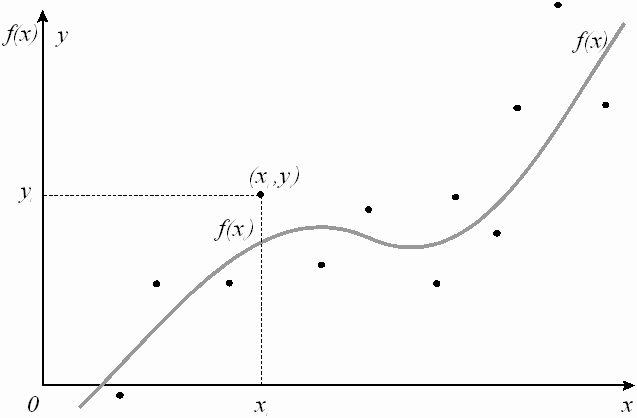
\includegraphics[width=.55\textwidth]{png/mnk.png}
		\caption{Пример нелинейной аппроксимации методом МНК}
		\label{mnk}
	\end{figure}

	\textbf{Примечание}. Рассмотренный ранее метод множественной линейной регрессии является по своей сути тоже частным случаем обобщения МНК на функции многих переменных. В рассматриваемых применениях эти методы различаются. Метод линейной регрессии предсказывает значения по другим параметрам, которые как-то могут характеризовать предсказываемую величину. МНК для временного ряда предсказывает параметр по набору предыдущих значений этого параметра.
	
\end{document}
